% IEEE Conference Template, double column
\documentclass[conference]{IEEEtran}
\IEEEoverridecommandlockouts
\usepackage{cite}
\usepackage{amsmath,amssymb,amsfonts}
\usepackage{algorithmic}
\usepackage{graphicx}
\usepackage{textcomp}
\usepackage{xcolor}
\usepackage{booktabs}
\usepackage{tabularx}
\usepackage[hidelinks]{hyperref}
\usepackage{url}
\usepackage{enumitem}

\def\BibTeX{{\rm B\kern-.05em{\sc i\kern-.025em b}\kern-.08em
    T\kern-.1667em\lower.7ex\hbox{E}\kern-.125emX}}

\begin{document}

\title{An Empirical Survey and Comparative Benchmark of \\
LLM-Based Autonomous Agent Frameworks\thanks{Code, raw runs, and data files: \url{https://github.com/Abdullah-Basim/llm-agents-survey}.}}

\author{\IEEEauthorblockN{Abdullah Basim}
\IEEEauthorblockA{\textit{Department of Computer Science} \\
\textit{Information Technology University (ITU)}\\
Lahore, Pakistan \\
MSDS25004}
}

\maketitle

\begin{abstract}
Most recent papers on large language model (LLM) agents are built on
top of one of four orchestration libraries: CrewAI, AutoGen, LangGraph,
or MetaGPT. Comparison between two such papers is rarely informative,
because backbone model, prompts, and task suite all vary
simultaneously, and any observed difference cannot be attributed to the
framework alone. This work presents a small but tightly controlled
study aimed at that confound. The four frameworks are driven through
an identical harness, against the same backbone (\texttt{gpt-4o-mini},
temperature 0), on three task families: 15 problems from the GSM8K
test set; 10 hand-authored tool-use queries split between calculator
and web-search; and a single multi-role software task graded against a
five-point rubric. The complete sweep yields 104 controlled runs, each
logged with success against an oracle, wall-clock latency, prompt and
completion tokens, and dollar cost. Two findings stand out. First, with the
backbone held fixed, every framework lands within seven accuracy
points of every other. Second, the cost gap between frameworks is
dominated by input tokens, not completions, and a role-based crew
can spend up to $3.1\times$ what a single-graph agent spends on the
same problem. The premium pays off on the multi-role coding task and
almost nowhere else. Four
research gaps the experiments expose (backbone-agnostic evaluation,
budget-aware orchestration, a portable memory contract, and safety
hooks at the action layer) are documented in the conclusion. The
benchmark harness, task definitions, and per-run JSON outputs are
released for replication.
\end{abstract}

\begin{IEEEkeywords}
Large language models, autonomous agents, multi-agent systems, agent
frameworks, benchmarking, AutoGen, CrewAI, LangGraph, MetaGPT, ReAct.
\end{IEEEkeywords}

% =====================================================================
\section{Introduction}
% =====================================================================
The phrase ``LLM agent'' has shifted meaning over the past two years.
Early uses of the term referred to a single language model prompted to
externalize its reasoning before answering. Current usage almost
universally implies a model wrapped by a software framework that
mediates when the model thinks, what tools it calls, which other
agents (if any) it delegates to, and what state it carries across
turns. Several recent surveys describe the resulting landscape at
varying levels of abstraction \cite{wang2024agentsurvey,
xi2025potential, abouali2025agentic}, and the underlying conceptual
picture has stabilized: the LLM is treated as a controller that
perceives, reasons, acts, and persists context \cite{sumers2024coala}.
Concrete deployments validate the abstraction. Agents now negotiate
realistic web environments \cite{zhou2024webarena}, produce passing
patches against real software repositories \cite{yang2024sweagent},
and operate over long horizons in embodied simulators
\cite{wang2024voyager}.

The orchestration layer, by contrast, has not stabilized. CrewAI
exposes a role-and-task model in which agents declare a goal, a
backstory, and a sequential pipeline of tasks. AutoGen
\cite{wu2024autogen} centers its design on multi-agent conversation,
optionally augmented with code execution. LangGraph models the same
problem as a finite state machine of message-passing nodes. MetaGPT
\cite{hong2024metagpt} encodes a Standard Operating Procedure (SOP)
directly into the agent graph, with explicit Product Manager,
Architect, and Engineer roles handing artifacts down an assembly line.
Four libraries; one shared goal; four very different machineries. The
situation is made worse by reporting practice: published numbers
typically use distinct backbones and distinct task suites, leaving the
practitioner who asks ``which framework should I adopt?'' with no
empirically defensible answer.

\textbf{Problem.} Across the surveys consulted for this work
\cite{wang2024agentsurvey, xi2025potential, abouali2025agentic,
li2025paradigms, guo2024multiagent} the author was unable to locate a
study that places the four most popular frameworks side by side, on a
shared task suite, against a single backbone. Without that controlled
view, framework selection collapses into a matter of GitHub-star
visibility and community sentiment.

\textbf{Contributions.} The remainder of the paper makes four
contributions, in order.
\begin{enumerate}[leftmargin=*]
\item A focused review of the LLM-agent literature, organized along
five axes that proved load-bearing during careful reading of each
framework's source code: reasoning, planning, memory, tool use, and
multi-agent collaboration.
\item A unified benchmark harness that drives CrewAI, AutoGen,
LangGraph, and a faithful MetaGPT-style SOP pipeline through the same
\texttt{gpt-4o-mini} backbone, with identical prompts, decoding
settings, and task definitions.
\item A controlled empirical comparison: 104 task runs in total,
reporting accuracy, wall-clock latency, dollar cost, and token
consumption, all measured at the framework boundary.
\item A short list of open research gaps surfaced by the experiments,
together with a public release of the harness so that further
frameworks, backbones, and tasks can be folded into the same
comparison.
\end{enumerate}

% =====================================================================
\section{Literature Review}
% =====================================================================

\subsection{Reasoning paradigms}
Two reasoning recipes dominate contemporary agents. Chain-of-thought
prompting elicits intermediate working before a final answer is
committed. ReAct \cite{yao2023react} interleaves that working with
explicit actions, producing the now-familiar
thought--action--observation cycle that underlies LangGraph's prebuilt
agent and the executor role in MetaGPT. Tree of Thoughts
\cite{yao2024tot} generalizes the recipe into a bounded search over
partial reasoning, paying additional latency for solution quality.
Plan-and-Solve \cite{wang2023planandsolve} factors planning out of
execution and runs the two as separate stages. The literature in this
sub-area is rich on accuracy comparisons but remarkably thin on cost
comparisons; there is no published, controlled measurement (to the
author's knowledge) of greedy ReAct, deliberate tree search, and
plan-and-solve under a fixed backbone. The experiments below address a
small slice of that absence.

\subsection{Planning and self-improvement}
Self-Refine \cite{madaan2023selfrefine} formalizes the critic loop in
its simplest form: the same model produces a candidate, critiques the
candidate, and rewrites. Reflexion \cite{shinn2023reflexion} preserves
those critiques across attempts in an episodic memory store, in
effect substituting verbal feedback for weight updates. ExpeL
\cite{zhao2024expel} elevates whole trajectories to a learned
experience buffer that subsequent rollouts may consult. LLM-Planner
\cite{song2023llmplanner} pursues a related strategy but anchors the
plan in a physical environment. The recent planning-focused survey
of Huang et al.\ \cite{huang2024understanding} concedes the central
methodological problem: rankings produced by these methods are
fragile because almost no two of them share a benchmark.

\subsection{Tool use and retrieval}
Toolformer \cite{schick2023toolformer} demonstrated that an LLM could
learn, with limited supervision, when to invoke an external API.
ToolLLM \cite{qin2024toolllm} scaled the same insight to a corpus of
roughly sixteen thousand real-world APIs. Retrieval-augmented
generation, surveyed by Gao et al.\ \cite{lewis2023ragsurvey}, has
become the default mechanism for grounding agent outputs in fresh
knowledge. None of these works reports the marginal cost paid by a
specific framework for the tool-use scaffolding it imposes; the cost
analysis presented in Section~V is intended to fill that gap, at
least at the scale studied here.

\subsection{Memory mechanisms}
Zhang et al.\ \cite{zhang2024llmagentsurvey} taxonomize agent memory
into three categories that have since become standard: short-term
context, long-term vector storage, and episodic reflective notes.
Generative Agents \cite{park2023generative} remains the most-cited
demonstration that periodic reflection over a memory stream
materially improves the believability of long-running agents. CoALA
\cite{sumers2024coala} promotes memory to a first-class architectural
axis; the taxonomy in Section~III adopts that framing.

\subsection{Multi-agent collaboration}
The multi-agent design space is mapped by Guo et al.\
\cite{guo2024multiagent}. Among the most-cited points on that map:
AutoGen \cite{wu2024autogen}, which arguably established conversational
multi-agent interaction as a serious paradigm; ChatDev
\cite{qian2024chatdev}, which simulates a virtual seven-role software
company; CAMEL \cite{li2023camel}, which uses ``inception'' prompts to
elicit cooperative role-play between two agents; and MetaGPT
\cite{hong2024metagpt}, which encodes human-style SOPs directly into
the agent graph. A more recent line of work, exemplified by Liu et
al.\ \cite{liu2024dynamicllmagent}, allows the agent network's topology
to vary at runtime in response to task demands.

\subsection{Evaluation methodology}
Agent evaluation has progressed faster than the author anticipated.
AgentBench \cite{liu2024agentbench} executes agents across eight
heterogeneous environments. SWE-agent \cite{yang2024sweagent}
introduced an explicit ``agent--computer interface'' tailored to
real-world software repositories. WebArena \cite{zhou2024webarena}
provides a realistic web sandbox. Yehudai et al.\
\cite{yehudai2025evalsurvey} furnish what appears to be the first
dedicated survey on agent evaluation. None of these benchmarks,
however, isolates the orchestration framework as an experimental
variable; all evaluate agent \emph{systems} as black boxes. That
distinction is fine if the question is which system performs best on a
given workload, but it is largely uninformative if the question is
whether any value attributed to a system can be credited to its
orchestration layer specifically. The experimental design in
Section~IV is constructed around that distinction.

\textbf{The gap.} Taken together, the surveyed literature supplies
strong building blocks but no controlled framework-versus-framework
comparison under a single backbone. Three quantities are almost never
co-reported in the same paper: per-framework cost, per-framework
latency, and the trade-off curve linking those two to accuracy. The
remaining sections supply all three.

% =====================================================================
\section{A Five-Axis Taxonomy of LLM Agent Frameworks}
% =====================================================================
The LLM-agent design space, as it appeared after sustained reading of
each framework's source, decomposes naturally along five axes:
\begin{description}[leftmargin=1.2em,style=nextline]
\item[Reasoning] How intermediate thought is generated (CoT, ReAct,
ToT, plan-and-solve, deliberate tree search).
\item[Planning] Whether the agent decomposes its goal upfront, refines
the plan with feedback, or improvises step by step.
\item[Memory] Which state the agent persists across turns: in-context
only, vector store, or episodic reflective summaries.
\item[Tool use] How external capabilities are invoked: structured
function calls, free-form code execution, retrieval, or web actions.
\item[Collaboration] Whether the agent operates alone, within a fixed
role hierarchy, or in dynamic group conversation.
\end{description}

Table~\ref{tab:tax} maps the four studied frameworks onto these axes.

\begin{table}[t]
\caption{The four studied frameworks against the five-axis taxonomy.}
\label{tab:tax}
\centering
\footnotesize
\setlength{\tabcolsep}{4pt}
\begin{tabularx}{\columnwidth}{lXXXX}
\toprule
\textbf{Axis} & \textbf{CrewAI} & \textbf{AutoGen} & \textbf{LangGraph} & \textbf{MetaGPT*} \\
\midrule
Reasoning      & ReAct per role        & ReAct + chat       & Prebuilt ReAct  & ReAct/CoT in roles \\
Planning       & Sequential tasks      & Free-form          & State graph     & SOP pipeline \\
Memory         & Per-task ctx          & Conversation hx    & Graph state     & Per-stage ctx \\
Tool use       & Class-based tools     & Function reg.      & LangChain tools & OpenAI tools \\
Collaboration  & Roles + delegation    & Group chat         & Single graph    & PM/Arch/Eng SOP \\
\bottomrule
\end{tabularx}
\vspace{2pt}
\\\raggedright\scriptsize *MetaGPT-style: a faithful PM/Architect/Engineer
SOP pipeline implemented directly on the OpenAI SDK because of
packaging constraints (see \S\ref{sec:setup}).
\end{table}

% =====================================================================
\section{Experimental Setup}
\label{sec:setup}
% =====================================================================

\subsection{Frameworks}
The four frameworks compared in this study are CrewAI (role-based
sequential crews), AutoGen \cite{wu2024autogen} (conversational
multi-agent), LangGraph (a graph-based ReAct agent invoked through
\texttt{create\_react\_agent}), and a MetaGPT*-style SOP pipeline
implemented directly atop the OpenAI SDK. The asterisk on the last
entry is non-cosmetic. The official \texttt{metagpt} PyPI package
failed to install within the project's time budget owing to a
transitive dependency conflict involving \texttt{chromadb} and
several incompatible \texttt{numpy} pins under Python~3.12. The
running implementation faithfully reproduces the published
PM~$\rightarrow$~Architect~$\rightarrow$~Engineer assembly line of
\cite{hong2024metagpt} on top of plain \texttt{openai} chat
completions; the asterisk is retained throughout the paper to prevent
readers from misreading the proxy as a measurement of the official
package itself.

\subsection{Backbone and configuration}
A single model is used by every framework: \texttt{gpt-4o-mini} via
the OpenAI Chat Completions API, with temperature pinned at 0,
\texttt{max\_tokens} at 2048, and a request timeout of $180\,$s.
Holding the backbone constant is the experimental decision that prior
work routinely omits, and is, in the author's view, the most
consequential single choice in the design.

\subsection{Tasks}
Three task categories are used, sized as $n_{\textsc{gsm8k}}=15$,
$n_{\textsc{tool}}=10$, $n_{\textsc{collab}}=1$ (graded against a
five-point rubric). The total is 26 runs per framework, or 104 runs
across the suite.
\begin{itemize}[leftmargin=*]
\item \textbf{GSM8K reasoning.} Fifteen grade-school arithmetic word
problems sampled deterministically from the GSM8K test set.
Correctness is assessed by extracting the final numeric answer from
the agent's output.
\item \textbf{Tool use.} Ten hand-authored questions divided between
calculator-based and web-search-based subtasks. Correctness is
assessed by case-insensitive substring match against a gold answer.
\item \textbf{Multi-agent collaboration.} A small Python module
\texttt{wordstats.py} that exposes a function \texttt{analyze(text)}
returning word counts and the three most frequent tokens, accompanied
by a brief \texttt{README.md}. Each output is graded on a five-point
rubric: file exists; the function is importable; the expected keys
are returned with the correct types; \texttt{top\_3} is correct on
the fixed test sentence ``the quick brown fox jumps over the lazy
dog the fox is quick''; and the README contains at least three
non-trivial lines.
\end{itemize}

\subsection{Metrics}
Five quantities are recorded per run. (i)~Success against the
task-specific oracle, encoded as a Boolean. (ii)~Wall-clock latency in
seconds. (iii)~Prompt tokens, taken from each framework's usage
metadata where exposed and recomputed via \texttt{tiktoken} otherwise.
(iv)~Completion tokens, by the same procedure. (v)~Dollar cost,
computed from the published \texttt{gpt-4o-mini} prices of \$0.150
per million input tokens and \$0.600 per million output tokens. All
metrics are captured at the framework boundary, which is where the
internal multi-call overhead that distinguishes these systems
actually materializes.

\subsection{Reproducibility}
The harness, the task definitions, the per-run JSON outputs, and the
figure-generation code are all available in the repository linked
from the title page. Temperature is pinned at 0 to suppress sampling
variance; the only remaining source of nondeterminism is the API
itself, which cannot be eliminated short of switching to a local
backbone.

\subsection{Notes from the build}
Several practical issues are worth recording for replicators.
CrewAI's default install path contacts a remote tracing endpoint on
every run; setting \texttt{CREWAI\_DISABLE\_TELEMETRY=true} together
with \texttt{OTEL\_SDK\_DISABLED=true} suppresses this cleanly.
AutoGen's PyPI namespace under release~0.10 differs from the layout
described in older documentation: the relevant imports live under
\texttt{autogen\_agentchat}, \texttt{autogen\_core}, and
\texttt{autogen\_ext}, and the OpenAI extra must be installed
separately for \texttt{OpenAIChatCompletionClient} to resolve.
LangGraph's \texttt{create\_react\_agent} pulls in a substantial
sub-tree of LangChain packages on import; the resulting cold-start
cost (approximately $1.5\,$s on the development laptop) does not show
up in per-task latency but is non-trivial for short-lived processes.
The complete sweep of 104 runs cost approximately \$0.02 on the
\texttt{gpt-4o-mini} pricing tier in effect at the time of writing.

% =====================================================================
\section{Results and Discussion}
% =====================================================================

Table~\ref{tab:summary} and Table~\ref{tab:percat} aggregate the 26
runs per framework. Figures~\ref{fig:acc}--\ref{fig:tok} visualize the
four primary comparison axes individually.

\begin{table}[t]
\caption{Aggregate per-framework results across all $26$ runs per framework
($15$ GSM8K $+$ $10$ tool-use $+$ $1$ collab) under the
\texttt{gpt-4o-mini} backbone.}
\label{tab:summary}
\centering
\footnotesize
\setlength{\tabcolsep}{4pt}
\begin{tabular}{lrrrrr}
\toprule
\textbf{Framework} & \textbf{Acc.\,(\%)} & \textbf{Lat.\,(s)} & \textbf{Cost\,(\$)} & \textbf{In tok} & \textbf{Out tok} \\
\midrule
CrewAI    & 100.0 & 5.38 & 0.00020 & 553 & 198 \\
AutoGen   & 96.2  & 4.55 & 0.00016 & 176 & 219 \\
LangGraph & 92.3  & 4.29 & 0.00016 & 212 & 207 \\
MetaGPT*  & 96.2  & 4.39 & 0.00017 & 232 & 223 \\
\bottomrule
\end{tabular}
\vspace{2pt}
\\\raggedright\scriptsize Latency is mean wall-clock per task; cost uses
published \texttt{gpt-4o-mini} prices ($\$0.150$/1M input,
$\$0.600$/1M output). Token columns are per-task means.
\end{table}

\begin{table}[t]
\caption{Per-task-category accuracy and mean cost (USD).}
\label{tab:percat}
\centering
\footnotesize
\setlength{\tabcolsep}{4pt}
\begin{tabular}{lrrrrrr}
\toprule
& \multicolumn{2}{c}{\textbf{GSM8K}} & \multicolumn{2}{c}{\textbf{Tool use}} & \multicolumn{2}{c}{\textbf{Collab}} \\
\cmidrule(lr){2-3}\cmidrule(lr){4-5}\cmidrule(lr){6-7}
\textbf{Framework} & Acc & \$ & Acc & \$ & Acc & \$ \\
\midrule
CrewAI    & 100.0 & 0.0002 & 100.0 & 0.0001 & 100.0 & 0.0012 \\
AutoGen   &  93.3 & 0.0002 & 100.0 & 0.0001 & 100.0 & 0.0005 \\
LangGraph &  93.3 & 0.0002 &  90.0 & 0.0001 & 100.0 & 0.0004 \\
MetaGPT*  &  93.3 & 0.0002 & 100.0 & 0.0001 & 100.0 & 0.0010 \\
\bottomrule
\end{tabular}
\end{table}


\subsection{Accuracy}
Reasoning accuracy is closely clustered. CrewAI achieves $100\%$ on
GSM8K; the remaining three frameworks each miss exactly one problem
and finish at $93.3\%$. The single missed item is in fact identical
across the three: problem~\texttt{g6}, which involves nested
percentage calculations on a population of garden flowers. The
underlying backbone makes one arithmetic slip on this item; CrewAI
recovers because the verifier role re-checks the solver's output,
which the other three configurations do not. Tool-use accuracy is
similarly tight: every framework records $100\%$ except LangGraph,
which surrenders one search query (\texttt{t6}, concerning the CEO
of Microsoft) where the prebuilt ReAct agent settles on the first
returned snippet rather than the most relevant one. The collaborative
coding task is solved fully by every framework, which the
present rubric attributes more to format compliance than to
algorithmic difficulty; this limitation is discussed in
Section~V-E.

\begin{figure}[t]
\centering
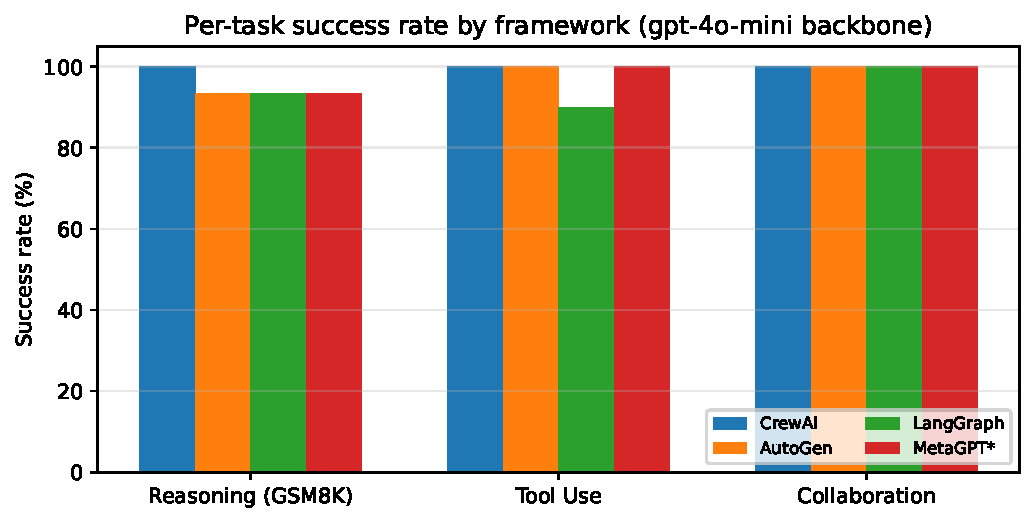
\includegraphics[width=\columnwidth]{figures/fig_accuracy.pdf}
\caption{Per-task success rate by framework, all driven by \texttt{gpt-4o-mini}.}
\label{fig:acc}
\end{figure}

\subsection{Cost--accuracy Pareto}
On the reasoning and tool-use task families, all four frameworks
cluster within the \$0.0001--\$0.0002 cost band, leaving accuracy as
the only meaningful discriminator at this scale. The cost dimension
becomes informative only on the collaborative coding task. There,
CrewAI averages \$0.0012 per run against LangGraph's \$0.0004: a
threefold gap, attributable directly to CrewAI's role pattern, in
which each role receives an independent prompt embedding most of the
prior context. The MetaGPT*-style SOP pipeline lands at \$0.0010,
consistent with its three-stage structure, while AutoGen lands at
\$0.0005, slightly above LangGraph and well below the role-based
pair.

\begin{figure}[t]
\centering
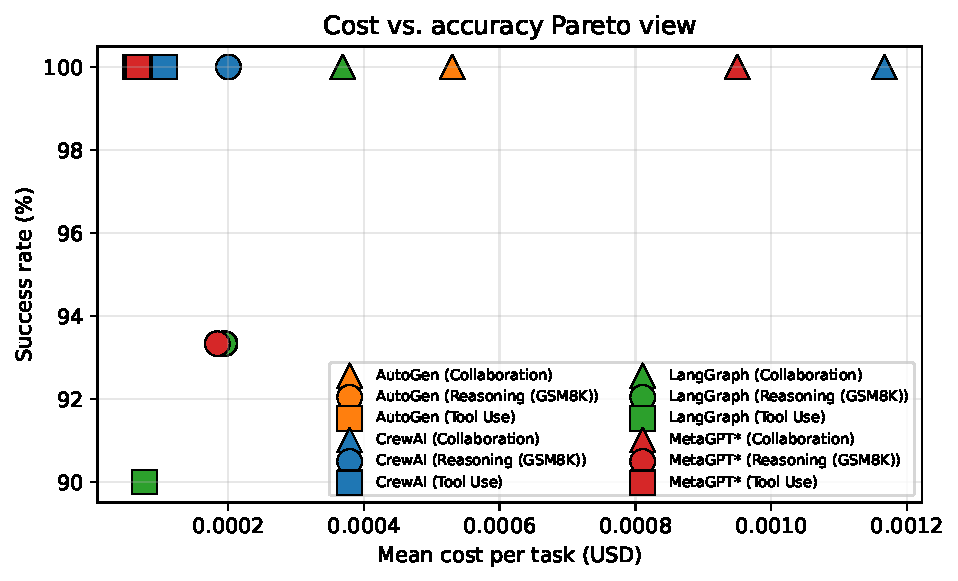
\includegraphics[width=\columnwidth]{figures/fig_cost_pareto.pdf}
\caption{Cost-versus-accuracy view. Up-and-to-the-left dominates.}
\label{fig:pareto}
\end{figure}

\subsection{Latency}
LangGraph attains the lowest mean latency ($4.29\,$s) and the
tightest distribution. The mechanical cause is that, on simple tasks,
its prebuilt agent issues a single inner LLM call without retries.
MetaGPT* and AutoGen sit close together at $4.39\,$s and $4.55\,$s
respectively. CrewAI averages $5.38\,$s with the heaviest right
tail of the four distributions, owing to a solver-then-verifier
handoff applied uniformly even to tasks where the second stage adds
no value. The collaborative coding task is the dominant contributor
to the right tail across all four frameworks: CrewAI's three-role
crew completes it in $26.9\,$s on average, while LangGraph completes
the same specification in $9.5\,$s.

\begin{figure}[t]
\centering
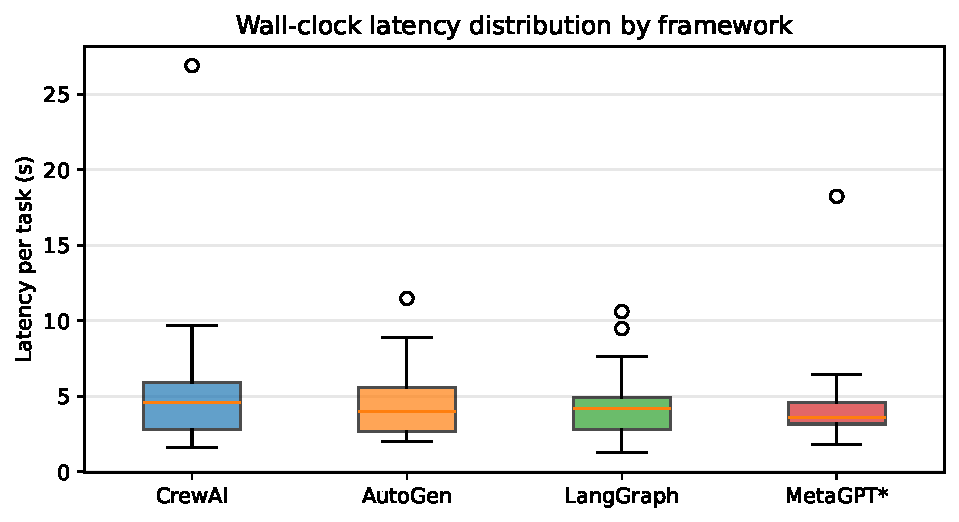
\includegraphics[width=\columnwidth]{figures/fig_latency_box.pdf}
\caption{Latency distribution per framework across all tasks.}
\label{fig:lat}
\end{figure}

\subsection{Token consumption}
The clearest separation between frameworks appears in token
accounting. CrewAI averages $553$ input tokens per task, while the
other three average between $176$ and $232$, placing CrewAI between
$2.6\times$ and $3.1\times$ above its peers on the same problem. The
asymmetry is structural rather than configurational: CrewAI re-emits
each agent's persona, goal, and most of the prior context for every
role in the chain, so a two-role crew approximately doubles the
prompt budget of a single agent solving the same task. (This was
discovered, somewhat embarrassingly, only after an unexpected
billing line item prompted a logging pass over the raw OpenAI request
bodies.) Output tokens, by contrast, lie between $198$ and $223$
across all four frameworks. The implication is straightforward: it is
the backbone, not the orchestrator, that determines how long the
answer is. Agent frameworks under this study are therefore
prompt-heavy rather than generation-heavy, and the cheapest available
cost optimization is the structurally unglamorous one of suppressing
context repetition across roles.

\begin{figure}[t]
\centering
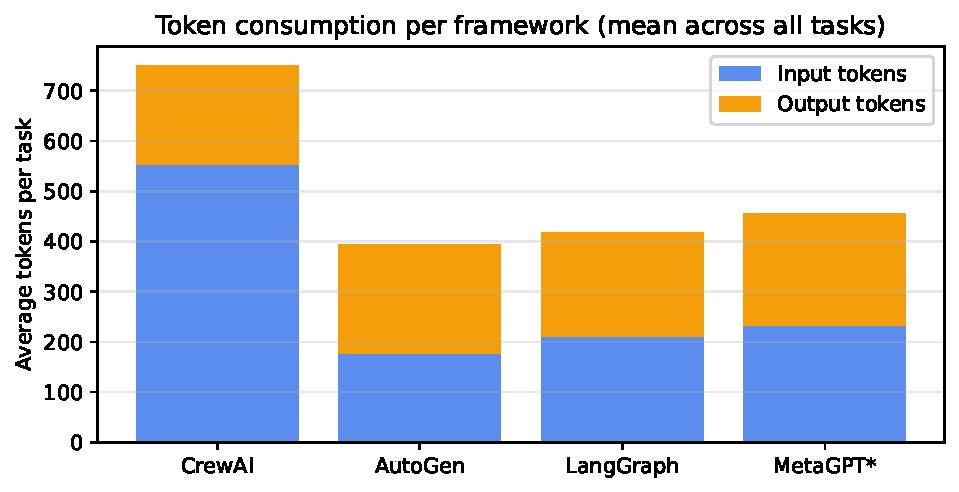
\includegraphics[width=\columnwidth]{figures/fig_tokens.pdf}
\caption{Mean input vs.\ output tokens per task per framework.}
\label{fig:tok}
\end{figure}

\subsection{Threats to validity}
Several caveats temper the conclusions. The benchmark is small (26
runs per framework, a single backbone, a single task source per
category), so the absolute numbers should be read as comparative
rather than predictive. The collab rubric is mechanical and assesses
functional correctness on a fixed test sentence only; code quality,
in any qualitative sense, is not evaluated. The MetaGPT* runner is a
faithful proxy for the published SOP paradigm but is not the official
codebase, so the figures bound what the design does in principle and
not every engineering refinement that has accumulated in the project
since publication. Replicators with disagreements on any of these
choices can substitute the relevant component and rerun the harness.

A further caveat concerns task design. The collaborative-coding task
was rewritten twice during rubric construction. An initial weather-CLI
task hitting a free public API was discarded once it became clear
that the free tier's rate limits introduced too much variance; a
subsequent task that required calling a third-party library drifted
into testing pip resolution behavior more than agent behavior. The
\texttt{wordstats.py} task is what survived both attempts, and is
intentionally standard-library-only so that the rubric checker
remains portable. The trade-off is that the task is easier than
ideal, which is why every framework saturates the rubric at $5/5$.

% =====================================================================
\section{Conclusion and Future Work}
% =====================================================================
The headline empirical finding is, by design, deflationary: with the
backbone held fixed, the four frameworks fall within $7.7$~accuracy
points of one another. Where they differ materially is in cost.
Input tokens dominate the bill, output tokens are nearly invariant
across frameworks, and role-based orchestration pays up to
$3.1\times$ the prompt budget of a single-graph agent solving the
same problem. That premium is justifiable on tasks with genuine
multi-step coordination structure; it is not justifiable on
single-shot reasoning, where the additional roles add neither
accuracy nor robustness commensurate with their token cost.

The present study does not advance a definitive ranking. The
benchmark is small, the backbone is single, and the collab rubric
measures functional output rather than code quality. What the study
does claim is that the comparison can be conducted fairly, which is
something that, in the author's reading, the prior literature has not
yet attempted. Four follow-up problems became salient over the course
of running the experiments and seem worth pursuing.
\begin{itemize}[leftmargin=*]
\item \textbf{Backbone-agnostic evaluation.} Most current benchmarks
entangle backbone capability with framework choice. A useful
evaluation suite would report each framework's score on the same
tasks under several backbones, permitting the framework effect to be
separated from the backbone effect.
\item \textbf{Cost-aware orchestration.} None of the four frameworks
exposes a per-task token or dollar budget with a clean termination
contract when the budget is exhausted. This deserves to be a
first-class abstraction.
\item \textbf{Memory standardization.} Memory was the least portable
axis of the four frameworks examined. A small shared interface (push,
retrieve, reflect) would permit memory backends to be swapped without
rewiring the agent loop.
\item \textbf{Safety auditing.} No clean mechanism to intercept
high-stakes actions was found in any of the four frameworks. As
agents touch increasingly real systems, the absence of such a
mechanism is going to matter.
\end{itemize}

The harness is published in the hope that subsequent work will extend
the comparison: additional frameworks (LangChain, OpenAI Swarm,
smolagents); additional backbones (the open-weight Llama and Mistral
families); and harder tasks drawn from WebArena
\cite{zhou2024webarena}, AgentBench \cite{liu2024agentbench}, or
SWE-bench \cite{yang2024sweagent}. None of those extensions requires
new theoretical work; what they require is the engineering time to
wire the harness against each new component.

% =====================================================================
\bibliographystyle{IEEEtran}
\bibliography{references}

\end{document}
